\documentclass[11pt]{article}
\usepackage{cth_course_template}
\usepackage{times}
\usepackage{url}
\usepackage{latexsym}
\usepackage{graphicx}
\usepackage{booktabs}

\aclfinalcopy % Uncomment this line for the final submission
%\def\aclpaperid{***} %  Enter the acl Paper ID here

\title{PA3: Sentiment Analysis System Report}

\author{Melker Gustafsson \\
  Chalmers \\
  {\tt melkergu@chalmers.se} \\\And
  Pontus Gideflod \\
  Chalmers \\
  {\tt pontusgi@chalmers.se} \\\And
  Ismail Sacic \\
  Chalmers \\
  {\tt ismails@chalmers.se} \\}

\date{}

\begin{document}
\maketitle
\begin{abstract}
This report outlines the development of a sentiment analysis system for \textit{Birch}. The project involved analyzing and cleaning a crowdsourced dataset, which contained significant noise due to inconsistent labeling. We implemented a machine learning pipeline to classify tweets into neutral, positive, or negative categories. We evaluated Logistic Regression, Linear SVC, and Naive Bayes classifiers, optimizing hyperparameters to maximize performance. The report compares these models against a baseline and discusses the impact of data quality on classification accuracy.
\end{abstract}
This report outlines the development of a sentiment analysis system for \textit{Birch}. The project involved analyzing and cleaning a crowdsourced dataset, which contained significant noise due to inconsistent labeling. A machine learning pipeline was implemented to classify tweets into neutral, positive, or negative categories. Logistic Regression, Linear SVC, and Naive Bayes classifiers were evaluated, with hyperparameters optimized to maximize performance. The report compares these models against a baseline and discusses the impact of data quality on classification accuracy.
\section{Introduction}
The objective of this project was to develop a text classification system capable of categorizing comments as neutral, positive, or negative. The system was built using existing training data provided by Birch. A key requirement for the project was transparency; the methodology and design choices needed to be clearly justifiable to facilitate future maintenance and development.

In this project, we focused on preprocessing the crowdsourced data to address quality issues, evaluating its reliability against a gold standard, and developing a robust classification model.

\section{Reflection on Annotation Task}

\subsection{Experience and Improvement Suggestions}
The annotation process presented several challenges, primarily regarding data consistency. A significant issue was spelling variations, as annotators entered labels manually (e.g., "postiv" vs "positive"). This necessitated a comprehensive data cleaning step.

 To improve future data collection, we suggest replacing the text input field with a predefined selection interface (such as radio buttons). This would eliminate typographical errors. Furthermore, using a single annotator per tweet is unreliable. We recommend employing multiple annotators (e.g., 3 or 5) for each data point and using a majority vote to determine the final label, thereby reducing individual bias.

\section{Data Exploration}

\subsection{Label Cleaning and Distribution}
The crowdsourced dataset contained inconsistent label formatting, including capitalization differences and spelling errors. We implemented a cleaning script to standardize all entries into three categories: neutral, positive, and negative.

Post-processing analysis revealed the following class distribution: 47.57\% neutral, 30.15\% positive, and 22.27\% negative. The dominance of the neutral class suggests potential challenges for the model, as class imbalance can bias predictions towards the majority class. Figure~\ref{fig:dist_crowd} illustrates this distribution.

\begin{figure}[htb]
\begin{center}
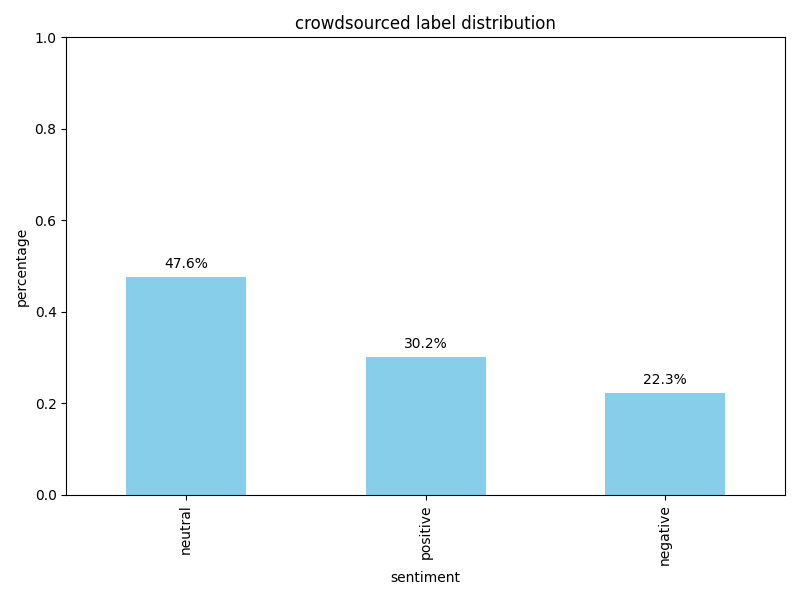
\includegraphics[width=75mm]{./graphics/distribution_crowdsourced.png}
\end{center}
\caption{Distribution of labels in the crowdsourced dataset.}
\label{fig:dist_crowd}
\end{figure}

\subsection{Comparison with Gold Standard}
To assess data reliability, we compared the crowdsourced labels against the "gold standard" dataset. The accuracy was approximately \textbf{65.5\%}. While this indicates moderate agreement, it highlights the presence of significant noise in the training data.

The confusion matrix (Figure~\ref{fig:agree_matrix}) shows that the primary source of disagreement was the 'neutral' class. Annotators frequently misclassified neutral tweets as positive or negative, indicating that the definition of neutrality is subjective and prone to interpretation variance.

\begin{figure}[htb]
\begin{center}
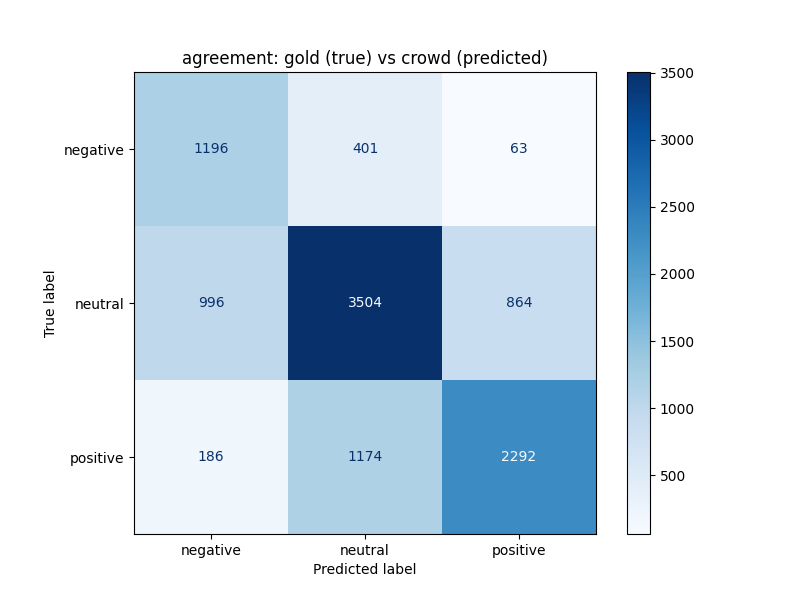
\includegraphics[width=75mm]{./graphics/confusion_matrix_agreement_gold_vs_crowd.png}
\end{center}
\caption{Confusion Matrix: Gold Standard (True) vs. Crowdsourced (Predicted).}
\label{fig:agree_matrix}
\end{figure}

\section{Classification System Implementation}

\subsection{Feature Representation and Processing}
We utilized the \texttt{TfidfVectorizer} from the Scikit-learn library to convert text data into numerical vectors. We employed Term Frequency-Inverse Document Frequency (TF-IDF) to weigh terms based on their importance, reducing the influence of common stop words. Additionally, we enabled \texttt{sublinear\_tf=True} to apply logarithmic scaling to term frequencies, which mitigates the impact of extremely high-frequency words.

\subsection{Model Selection and Method Choices}
To establish a strong baseline, we prioritized linear models over complex architectures. We evaluated three classifiers: Logistic Regression, Linear SVC (Support Vector Classifier), and Multinomial Naive Bayes. Linear models typically perform well on high-dimensional sparse data such as text. We used 5-fold cross-validation with \texttt{GridSearchCV} to optimize hyperparameters, ensuring the results were robust and not dependent on a specific data split.

\subsection{Evaluation and Results}
We compared model performance against a "Dummy" baseline that predicts the majority class (Neutral).

\subsubsection{Performance on Crowdsourced Data}
The Linear SVC model achieved the highest performance during cross-validation. Figure~\ref{fig:res_crowd} presents the confusion matrix for this model.

\begin{figure}[htb]
\begin{center}
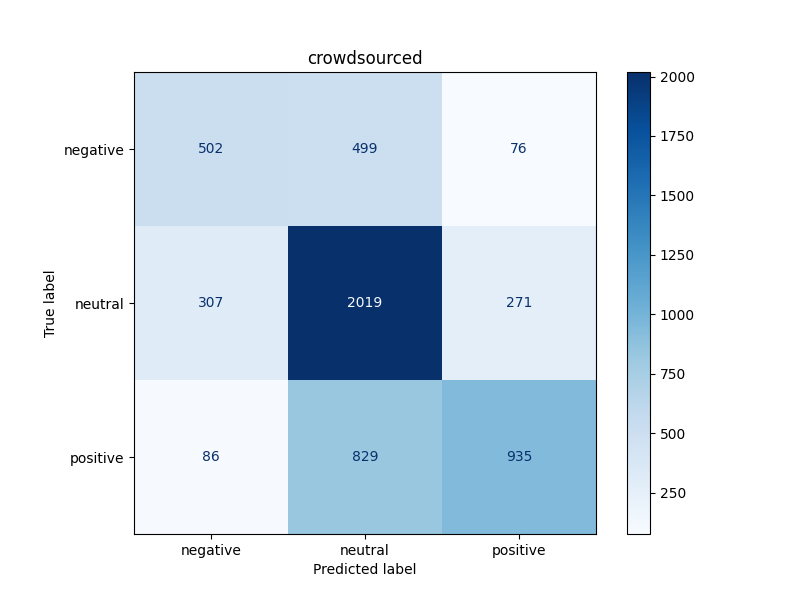
\includegraphics[width=75mm]{./graphics/confusion_matrix_result_crowdsourced.png}
\end{center}
\caption{Confusion Matrix for the classifier trained on Crowdsourced data.}
\label{fig:res_crowd}
\end{figure}

The baseline accuracy was \textbf{47.57\%}, while our best model achieved approximately \textbf{63.05\%}. Although this represents a significant improvement, the confusion matrix indicates persistent errors in distinguishing the 'neutral' class, likely stemming from the inconsistencies observed in the training data.

\subsubsection{Performance on Gold Standard Data}
We retrained the model using the gold standard dataset to evaluate the impact of label quality.

\begin{figure}[htb]
\begin{center}
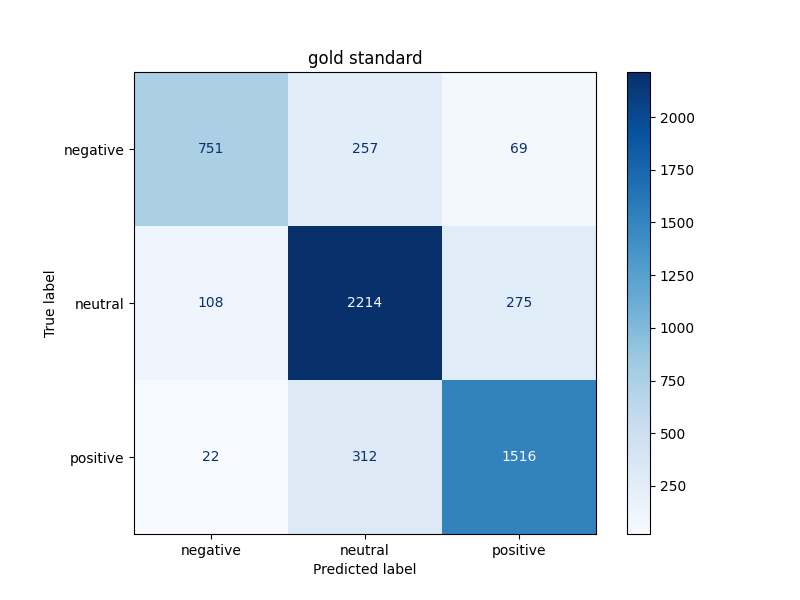
\includegraphics[width=75mm]{./graphics/confusion_matrix_result_gold_standard.png}
\end{center}
\caption{Confusion Matrix for the classifier trained on Gold Standard data.}
\label{fig:res_gold}
\end{figure}

With the high-quality data, accuracy improved to \textbf{66.6\%}. This confirms that label noise in the crowdsourced data negatively affects performance. However, the moderate improvement suggests that the task of distinguishing sentiment from neutrality remains inherently difficult using bag-of-words approaches.

\section{Discussion and Future Work}

\subsection{Error Analysis}
The system's primary weakness is the classification of 'neutral' tweets. Both human annotators and the model struggle with this category. The model often misinterprets the presence of sentiment-bearing words as an indicator of positive or negative polarity, even when the overall context is neutral.

\subsection{Prioritization and Constraints}
Due to time constraints, we prioritized establishing a reliable processing pipeline and analyzing data quality over implementing complex deep learning models. We focused on data cleaning to address the identified label noise, as this was deemed critical for model performance.

\subsection{Future Recommendations for Birch}
To improve system performance, we recommend clarifying the annotation guidelines, particularly for the 'neutral' class, to reduce subjectivity. We also suggest exploring Deep Learning approaches, such as BERT, which can capture context and nuance better than frequency-based models. Finally, collecting additional data for the minority 'negative' class would help address class imbalance.

\section{Conclusion}
We have developed a text classification system for Birch that effectively handles noisy crowdsourced data. Our evaluation identifies Linear SVC as the most effective model for this task. The analysis highlights that the ambiguity of 'neutral' tweets is the main bottleneck for performance. While the current system outperforms the baseline, significant improvements would likely require higher-quality training data and clearer annotation protocols.
